\section{Implementation, integration and testing plan}
This section will be dedicated to discuss how the subcomponents' implementation is planned, to present the integration plan and then
to explain the tests dedicated to evaluate if the System behaviours as expected. 
\subsection{Development Process and Approach}
The application is composed of three layers (client, business and data) and these layers can be implemented in parallel and integrated.
The tiers can be unit tested independently and after the integration they can be tested at the end as the whole System.
The whole System can be implemented, integrated and tested exploiting bottom-up approach. The decision to use this approach derives
from the possibility to incrementally develop the system by proceeding implementing in parallel the different tiers. 
The components are tested and integrated with other components to evaluate the dependencies between components of the same subsystem.

\subsubsection{Frontend}
It consists of the PWA and web application for the EV Drivers and the web application for CPOs that can be developed and tested independently
since are decoupled and doesn't communicate directly. Both the two components rely on REST API to interact with the business logic and can be unit tested by mocking 
the REST APIs. 
\subsubsection{Backend}
It consists of business logic and the data logic. The application server of the business logic is composed by the Query Manager and two important components,
the eMSP and the CPMS that need to communicate each other. The developers can be work separately on 
eMSP and CPMS and integrate and test at the end of their development the two components to evaluate the dependency and the interactions between them.
These whole business logic can be tested independently from the client logic, speeding up the development process. 
In the following two sections will be analyzed the complexity and the importance for the subcomponents of the eMSP and the CPMS.
\\
\begin{itemize}
    \item \textbf{eMSP} \\ In the following two sections will be analyzed the complexity and the importance for the subcomponents of the eMSP.
    
    \begin{center}
        \begin{tabular}{|p{6cm}|l|l|}
            \hline
            \textbf{Component} & \textbf{Importance} & \textbf{Complexity}\\
            \hline
            Account Manager & High & Medium \\
            \hline
            CP Search Manager & High & Medium \\
            \hline
            Car Manager & Medium & Medium \\
            \hline
            Reservation Manager & High & High \\
            \hline
            Suggestion Manager & Medium & Medium \\
            \hline
            Notification Manager & Medium & Medium \\
            \hline
            eMSPtoCPMSConnector & High & High \\
            \hline
            Query Manager & High & Low \\
            \hline
         \end{tabular}
    \end{center}
    \noindent \\
    \item \textbf{CPMS} \\ In the following two sections will be analyzed the complexity and the importance for the subcomponents of the CPMS.
    
    \begin{center}
        \begin{tabular}{|p{6cm}|l|l|}
            \hline
            \textbf{Component} & \textbf{Importance} & \textbf{Complexity}\\
            \hline
            Account Manager & High & Medium \\
            \hline
            Rate Manager & Medium & Low \\
            \hline
            Energy Manager & Medium & Medium \\
            \hline
            Reservation Manager & High & High \\
            \hline
            Charging Points Manager & High & High \\
            \hline
            Query Manager & High & Low \\
            \hline
         \end{tabular}
    \end{center}
    \noindent \\
\end{itemize}

\subsubsection{External components} 
All the external APIs are provided by third parties and are supposed to be reliable and conform to their specification. 

\subsection{Implementation Plan}
The implementation of the Application Server will be divided between eMSP and CPMS a can be done in parallel.
\subsubsection{eMSP}
\begin{enumerate}
    \item \textbf{Query Manager}: It is the first component to be implemented since all the other component relies on This
    on to interact with the Database. It is the only component in which is necessary to implement the queries to the database.
    \item \textbf{Notification Manager}: Then component can be implemented, it offers two interfaces to two components that will later 
    be developed.
    \item \textbf{Account Manager}: This is the component that permits to register or log in a user. It has an authorization interface that 
    is used by the other components to verify at each request that the user has the permissions to do the requested operations.
    \item \textbf{eMSPtoCPMSConnector}: The development of this module is particularly critic because is the component dedicated
    to the communication with the CPMS. The dialogue between the two can be simulated during the implementation and tested after the integration.
    \item \textbf{Charging Points Manager, Reservation Manager, Suggestion Manager, Car Manager}: These components can be implemented
    in parallel since there are no dependencies between them. 
\end{enumerate}
\subsubsection{CPMS}
\begin{enumerate}
    \item \textbf{Query Manager}: It is the first component to be implemented since all the other component relies on This
    on to interact with the Database. It is the only component in which is necessary to implement the queries to the database.
    \item \textbf{Account Manager}: This is the component that permits to register or log in a user. It has an authorization interface that 
    is used by the other components to verify at each request that the user has the permissions to do the requested operations.
    \item \textbf{CPMStoeMSPConnector}: The development of this module is particularly critic because is the component dedicated
    to the communication with the eMSP. The dialogue between the two can be simulated during the implementation and tested after the integration.
    \item \textbf{Rates Manager}: This component has to be implemented before the Charging Points Manager because during the adding 
    of a new CP to the Manager, a rate needs to be associated to the CP.
    \item \textbf{Charging Points Manager and Reservation Manager}: These two components are the most critical to implement but also two 
    of the most essential components. The dialogue between the CPMS and the CPs is done through the Charging Points Manager that 
    needs to be implemented compliant with the OCPP protocol used by the CPs. The Reservation Manager on the other hand is the component
    that manages all the reservation done through the eMSP to the specific CPMS. These two components can be implemented in parallel.
    \item \textbf{Energy Manager}: This component has a medium complexity because it interacts with the DSO Pricing Service and Energy Storage API. 
\end{enumerate}

\subsection{Integration Plan}
The section describes the integration plan of the different components and subcomponents of the eMAll System. 
The graphs below show the dependencies of a component or subcomponent on another component or subcomponent. Each subcomponent before being integrated with others subcomponents
to form a component need to be unit tested and after the integration the integrated component will be tested.
The testing can be done in parallel between eMSP and CPMS.
\subsubsection{eMSP}
The first components to be tested together are the Query Manager and the DBMS as they are the components necessary for all the others when handling data.
\begin{figure}[H]
    \centering
    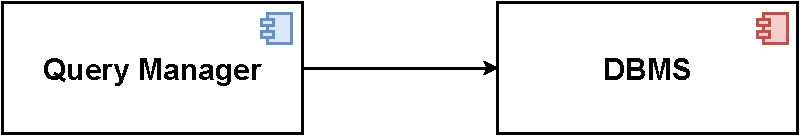
\includegraphics[scale=0.6]{src/Integration/eMSPQuery.pdf}
    \caption{Data Subsystem}
\end{figure}
Before implementing the Account Manager it is preferred to develop the Notification Manager.
\begin{figure}[H]
    \centering
    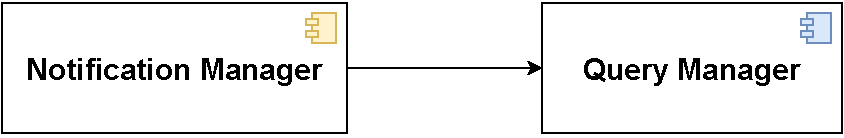
\includegraphics[scale=0.6]{src/Integration/eMSPNotification.pdf}
    \caption{Notification Subsystem}
\end{figure}
Then it can be implemented the Account Manager that provides the account managing functions and the authorization interface 
to verify the permissions to do operations with the other components. It handles personal user's data and for this reason needs
to be tested carefully.
\begin{figure}[H]
    \centering
    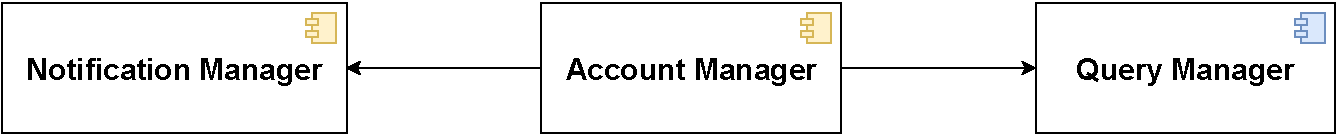
\includegraphics[scale=0.6]{src/Integration/eMSPAccount.pdf}
    \caption{Account Subsystem}
\end{figure}
The eMSPtoCPMSConnector can be implemented after the Account Manager, a stub of the CPMS can be implemented at this point to simulate
the response of the CPMS on the other side of the communication. This stub is an exception to the bottom-up approach, but
enables the possibility to develop separately the eMSP and the CPMS.
\begin{figure}[H]
    \centering
    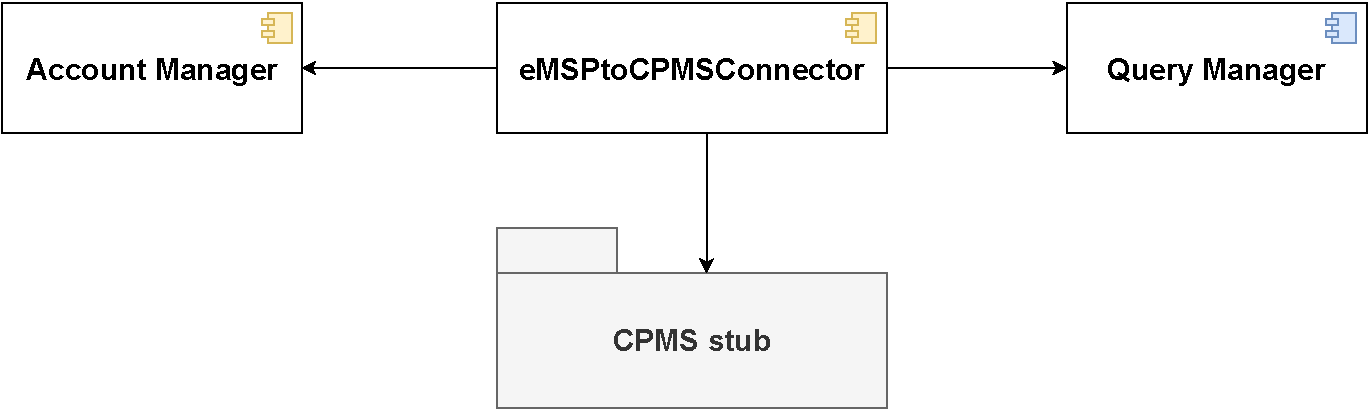
\includegraphics[scale=0.6]{src/Integration/eMSPConnector.pdf}
    \caption{Connector Subsystem}
\end{figure}
Then the following subsystems could be developed in any order or in parallel because they are decoupled. All the components require
the eMSPtoCPMSConnector to simulate and test efficiently the implementation. 
The develop can start from the most complex tasks such as the Charging Point Manager and the Reservation Manager. 
Then the Suggestion Manager and the Car manager can be implemented.
\begin{figure}[H]
    \centering
    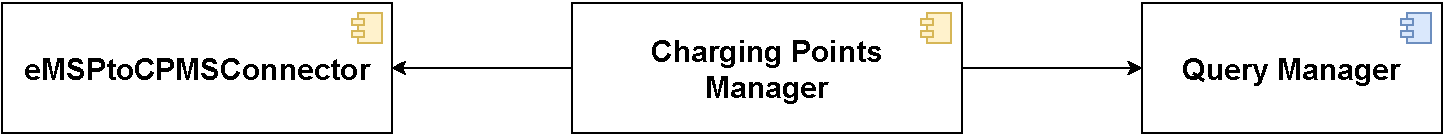
\includegraphics[scale=0.6]{src/Integration/eMSPCP.pdf}
    \caption{Charging Points Subsystem}
\end{figure}
\begin{figure}[H]
    \centering
    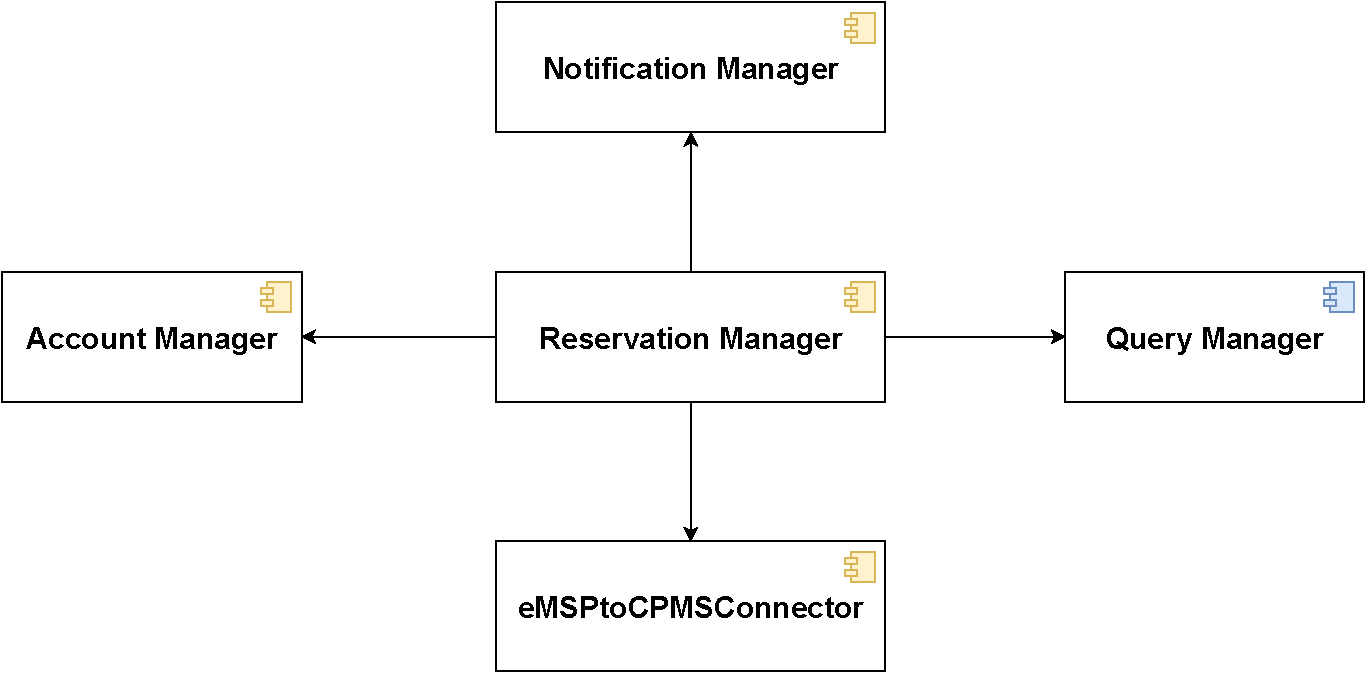
\includegraphics[scale=0.6]{src/Integration/eMSPReservation.pdf}
    \caption{Reservation Subsystem}
\end{figure}
\begin{figure}[H]
    \centering
    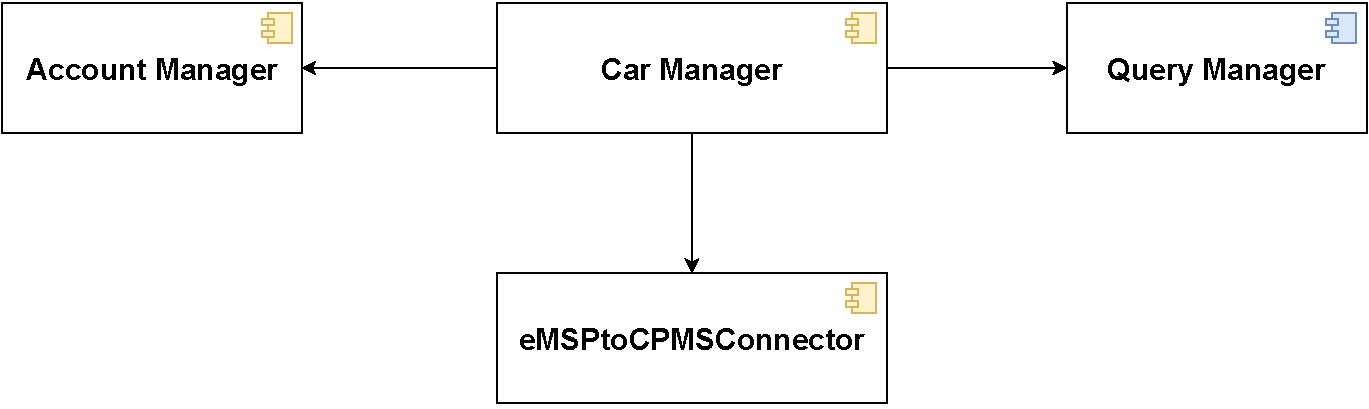
\includegraphics[scale=0.6]{src/Integration/eMSPCar.pdf}
    \caption{Car Subsystem}
\end{figure}
\begin{figure}[H]
    \centering
    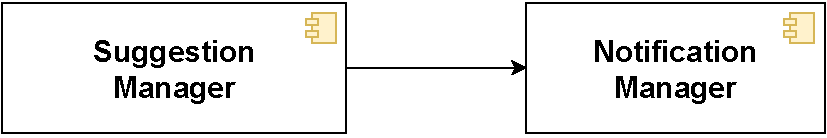
\includegraphics[scale=0.6]{src/Integration/eMSPSuggestion.pdf}
    \caption{Suggestion Subsystem}
\end{figure}
After having implemented and tested all the subsystems, the client and the eMSP can be integrated 
and tested together. 
\begin{figure}[H]
    \centering
    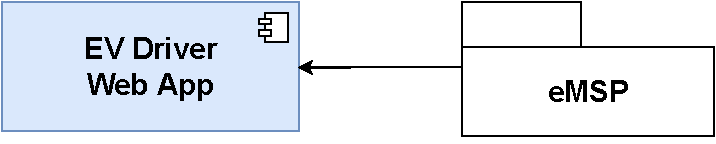
\includegraphics[scale=0.6]{src/Integration/eMSPFrontend.pdf}
    \caption{Client Application Integration}
\end{figure}


\subsubsection{CPMS}
The first components to be tested together are the Query Manager and the DBMS as they are the
components necessary for all the others when handling data.
\begin{figure}[H]
    \centering
    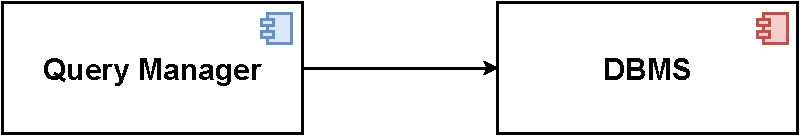
\includegraphics[scale=0.6]{src/Integration/CPMSQuery.pdf}
    \caption{Data Subsystem}
\end{figure}
Then it can be implemented the Account Manager that provides the account managing functions and the authorization interface 
to verify the permissions to do operations with the other components. It handles personal CPO's data and for this reason needs
to be tested carefully.
\begin{figure}[H]
    \centering
    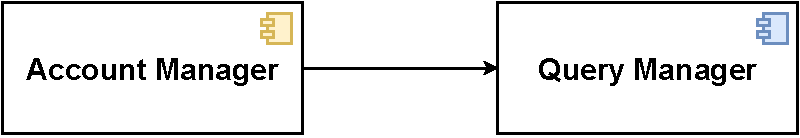
\includegraphics[scale=0.6]{src/Integration/CPMSAccount.pdf}
    \caption{Account Subsystem}
\end{figure}
The CPMStoeMSPConnector can be implemented after the Account Manager, a stub of the eMSP can be implemented at this point to simulate
the requests coming from the eMSP on the other side of the communication. This stab is an exception to the bottom-up approach, but
enables the possibility to develop separately the eMSP and the CPMS. 
\begin{figure}[H]
    \centering
    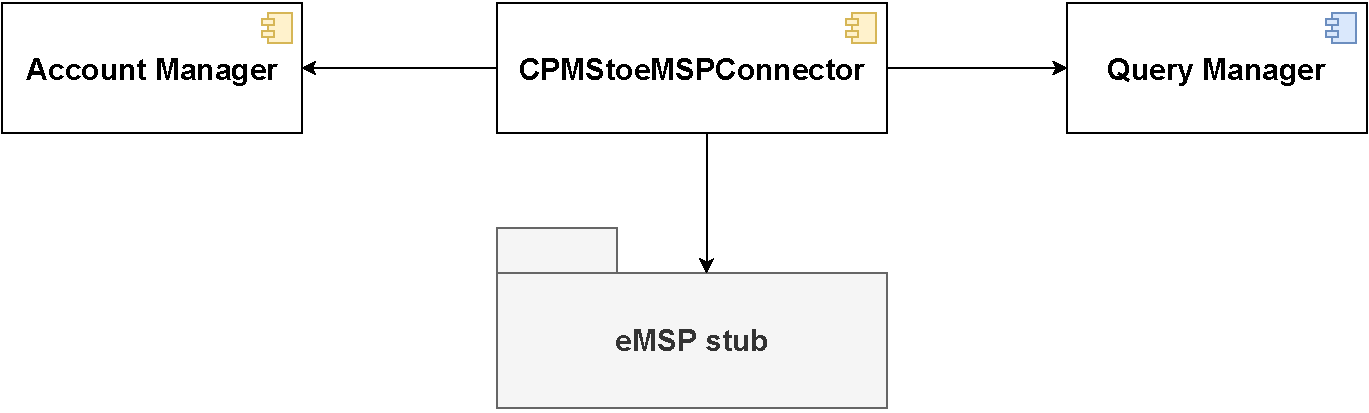
\includegraphics[scale=0.6]{src/Integration/CPMSConnector.pdf}
    \caption{Connector Subsystem}
\end{figure}
Then can be implemented the Rates Manager that offers an interface to create and modify rates that
are later associated with the CPs.
\begin{figure}[H]
    \centering
    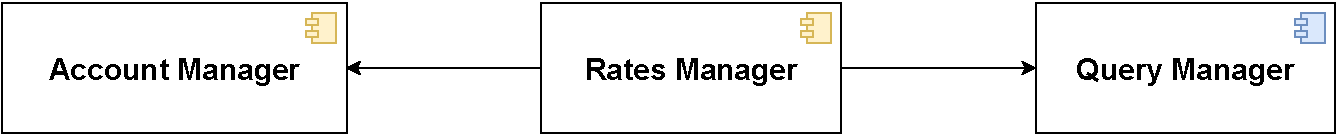
\includegraphics[scale=0.6]{src/Integration/CPMSRates.pdf}
    \caption{Rates Subsystem}
\end{figure}



\subsection{System Testing}
Eventually, when the integration of the components have taken place take place the testing of the entire System. 
The aim is to verify the functional and non-functional requirements and must take place in a testing
environment that is as close as possible to the production environment. 
The eMall System will undergo the following test:
\begin{itemize}
    \item \textbf{Functional testing}: The system is tested against the functional requirements and specification 
    specified on the RASD document.
    \item \textbf{Performance testing}: Check wether a software remains functional with increase demand and 
    various environment conditions.
\end{itemize}
